% Supplementary Information
% Compile with: pdflatex supplementary.tex   (twice)
\documentclass{article}

\PassOptionsToPackage{numbers,compress}{natbib}
\usepackage[preprint,nonatbib]{neurips_2026}

\usepackage[utf8]{inputenc}
\usepackage[T1]{fontenc}
\usepackage{lmodern}
\usepackage{hyperref}
\usepackage{xurl}
\usepackage{booktabs}
\usepackage{array}
\usepackage{ragged2e}   % RaggedRight keeps hyphenation inside p-columns
\usepackage{amsfonts}
\usepackage{amsmath}
\usepackage{amssymb}
\usepackage{microtype}
\usepackage{graphicx}
\graphicspath{{../}}

\usepackage{caption}
\DeclareCaptionLabelSeparator{nature}{ \textbar\ }
\captionsetup{font=small,labelfont=bf,labelsep=nature,
              justification=justified,singlelinecheck=false}
\renewcommand{\figurename}{Supplementary Figure}
\renewcommand{\tablename}{Supplementary Table}

\setlength{\emergencystretch}{2em}

\title{Supplementary Information\\[6pt]
\large Recognizing the predictive boundary of\\historically restricted physical knowledge}

\author{%
  Chenxi He \\ Cavendish Laboratory, University of Cambridge \\
  \And
  Jingqiu Chen \\ Shenzhen University \\
}

\begin{document}
\maketitle

EPOCH: Epistemic Probe Of Classical Horizons.

\section{Supplementary Note 1: Protocol status and confirmatory design}

The historical experiments are retrospective rather than pre-registered. The analysis protocol fixes the interior rule, frontier fraction (0.30), dictionary \{power, exponential, linear, constant\}, precision floors and random seeds within the analysis archive. Its 0.5 percentile rule is an exploratory alert threshold corresponding to the median calibration score, not a statistical rejection threshold. A confirmatory design freezes a primary threshold at 5\% FPR and a secondary threshold at 1\% FPR on an independent calibration set before a sealed test set is opened. It reports finite-sample upper-tail probabilities with calibration ties counted conservatively and apply BH false-discovery-rate control when multiple datasets are scanned. The timestamped protocol covers task routing, exclusion criteria, data transformations, measurement models, boundary intervals and abstention rules.

Every test must instantiate \(\mathcal{T}=(\mathcal{M},\Theta,P_\varepsilon,I,A,S,\alpha)\): admissible models, fitted parameters, observation/censoring model, fitting-eligible data, the complete adaptive algorithm, the final statistic and the error rate. Direction choice, window search, model selection and parameter fitting are part of \(A\) and must be rerun inside every null/calibration replicate. The four allowed semantic outputs are \emph{compatible over the measured range}, \emph{localized model incompatibility}, \emph{whole-range model incompatibility without an identifiable boundary} and \emph{insufficient evidence / abstain}. ``Established theory fails'' is permissible only if the declared model set is an adequate encoding of that theory's relevant prediction; failure of the four-form dictionary alone does not license that interpretation.

\section{Supplementary Note 2: The extrapolation-residual ratio (definition and invariances)}

For data $(x,y)$, the best classical form $f$ from the dictionary is fitted on the interior and extrapolated to the frontier. With log-residuals $r(x)=\lvert\log(\lvert y\rvert/\lvert f(x)\rvert)\rvert$, the statistic is

\[
\text{extrapolation-residual ratio}=\frac{\operatorname{median}_{\text{frontier}} r}{\operatorname{median}_{\text{interior}} r}.
\]

Empirical invariance tests show that the ratio is unchanged under $y\to a\,y$ (amplitude) and $x\to b\,x$ (units), and remains robust to additive noise up to 5--10\%. The companion statistic, called the split-conformal nonconformity in the main text, is the mean absolute frontier residual divided by the 90th percentile of the interior residuals, with the same one-percent relative floor; it is a scaled frontier residual and carries no coverage guarantee of its own. The ratio is an ordinal breakdown indicator. Reported magnitudes, including the FIRAS over-prediction factor, therefore include a window-dependence range and bootstrap confidence interval.

\section{Supplementary Note 3: Detector benchmark and anti-circularity ablation}

The head-to-head benchmark and learned-component comparison use separate suites. The anti-circularity ablation varies the information supplied on the benchmark phenomena.

\subsection{Head-to-head benchmark}

On the fair synthetic suite ($n = 36$; needs-new versus classical; Supplementary Fig.~1d), AUROC is reported with overlapping bootstrap 95\% confidence intervals of approximately $\pm 0.13$.

\begin{table}[htbp]
\centering
\caption{\textbf{Head-to-head detector benchmark on the 36-dataset fair suite.}}
\small
\begin{tabular}{@{}lr@{}}
\toprule
Method & AUROC \\
\midrule
statistical detector (conformal + breakdown ratio) & 0.80 \\
split-conformal & 0.77 \\
Ramsey RESET F-test & 0.73 \\
extrapolation-residual (breakdown) ratio & 0.72 \\
CUSUM change-point & 0.67 \\
Gaussian-process model discrepancy & 0.58 \\
\bottomrule
\end{tabular}
\end{table}

\subsection{Anti-circularity ablation}

The ablation measures AUROC on the same phenomena while varying the information supplied by the analyst.

\begin{table}[htbp]
\centering
\caption{\textbf{Anti-circularity ablation on the same phenomena.}}
\small
\begin{tabular}{@{}lr@{}}
\toprule
Condition & AUROC \\
\midrule
classical law given & 1.00 \\
law auto-selected from dictionary & 1.00 \\
law and interior regime withheld (auto-selected) & 0.97 \\
\bottomrule
\end{tabular}
\end{table}

Automatic selection of both the classical law and its regime retains AUROC 0.97 on this suite. On a separate 180-dataset suite, the deformation-supervised learned probe reaches AUROC 0.83 compared with 0.62 for its statistical comparator. The probe was trained on breakdown morphologies, so this gap measures morphology supervision rather than classical-only recognition.

\begin{figure}[htbp]
  \centering
  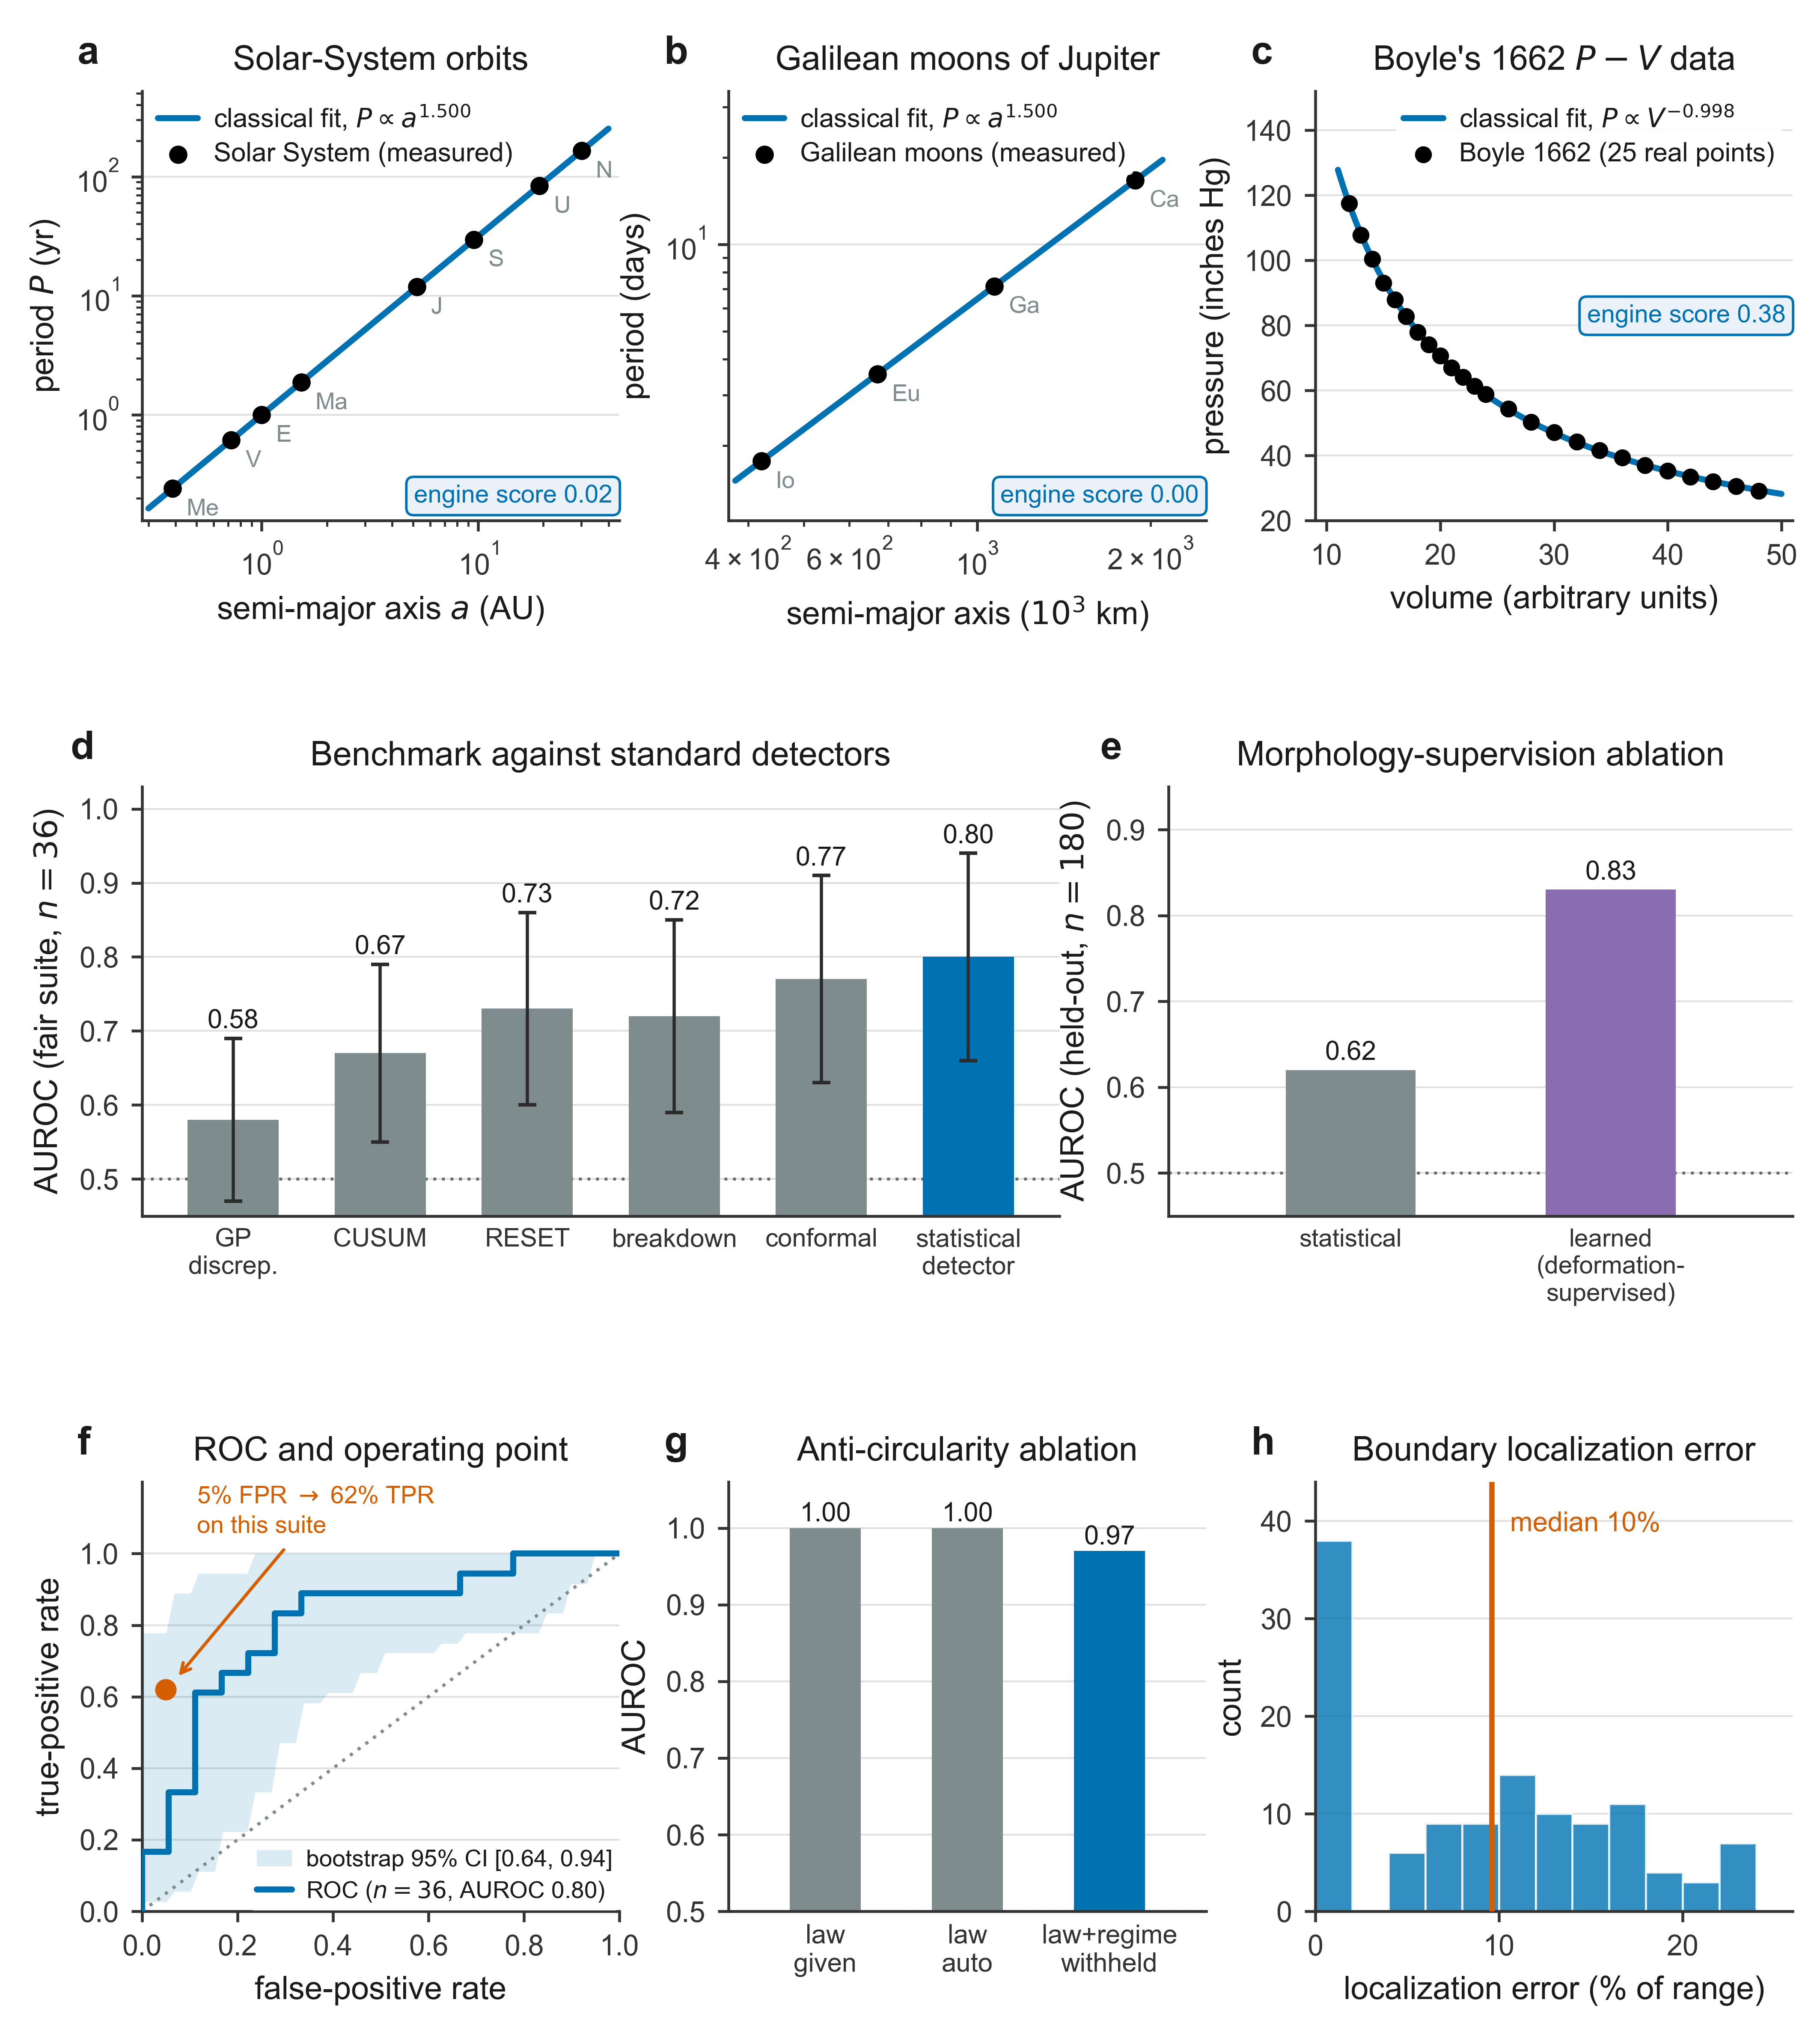
\includegraphics[width=\textwidth,keepaspectratio]{figures/figure_benchmarks.png}
  \caption{\textbf{Measured classical controls, synthetic benchmarks and
  ablations. a--c}, Solar-System orbits, the Galilean moons and Boyle's 1662 pressure--volume table recover their expected exponents and score 0.02, 0.00 and 0.38, below the 0.5 screening threshold. \textbf{d}, AUROC on the 36-dataset fair suite against Gaussian-process discrepancy, CUSUM, RESET, a breakdown comparator and split-conformal prediction, with bootstrap 95\% intervals. \textbf{e}, On the 180-dataset suite the deformation-supervised probe reaches AUROC 0.83 against 0.62 for its statistical comparator; the positive-only probe reaches 0.453 against 0.695 on the same suite, which isolates what anomaly-morphology supervision contributes. \textbf{f}, ROC on the fair suite with a bootstrap 95\% band; TPR at 5\% FPR is 62\% here and 27\% on the mechanism-level audit, which resamples by mechanism family rather than by realization. \textbf{g}, Anti-circularity ablation: AUROC is 1.00 when the classical law is given, 1.00 when it is selected automatically and 0.97 when both law and interior are selected automatically. \textbf{h}, Point localization error on synthetic onsets; calibrated interval coverage is evaluated separately in Fig.~5c.}
  \label{sfig:benchmarks}
\end{figure}

\section{Supplementary Note 4: Confidence intervals, false-positive rate and strict evidence audit}

The statistical detector reaches AUROC 0.80 with bootstrap 95\% CI [0.64, 0.94], resampled over 36 synthetic phenomena. The 62\% TPR at 5\% FPR belongs to this narrow suite. In the broader mechanism-level benchmark, an uncapped log score is calibrated separately at $n = 5$, 9, 43 and 120 using 785 valid classical simulations per size. Across 12 alternative mechanism families with eight realizations each, TPR is 0.271 at the calibration-targeted 5\% FPR (mechanism-bootstrap 95\% CI [0.073, 0.500]) and 0 at the targeted 1\% FPR. On a separate synthetic clean-null set of 12 classical function families with eight realizations each, the realized FPR is 0/96 at both thresholds; neither class has a fit failure or abstention. This null is synthetic and independent of the calibration set. The formula-derived frozen evaluation (200 formula point clouds and 30 synthetic breakdowns) reaches AUROC 0.88, recall 0.90 and false-positive rate 0.24 at the exploratory median threshold.

The strict real-case audit used 392 valid scores from 400 requested classical calibration records. With the capped statistic, FIRAS, copper specific heat, Bertozzi and Onnes have finite-sample upper-tail p-values 0.053, 0.053, 0.346 and 0.346. Their BH q-values are 0.107, 0.107, 0.346 and 0.346. The statistic reaches its hard ceiling for approximately 5\% of full-size and 34\% of small-size classical calibration datasets, preventing stronger evidence. A diagnostic uncapped log-combination gives nominal p-values 0.031, 0.023, 0.176 and 0.173, but none survives four-case BH control. The uncapped combination was examined after the capped result and is reported as a design diagnostic.

\section{Supplementary Note 5: Real-data details}

\begin{description}
\item[COBE-FIRAS.] The 43-point NASA LAMBDA published spectrum
(\nolinkurl{firas_monopole_spec_v1.txt}; Fixsen et al.~1996) spans
$x = h\nu/kT \in [1.2, 11.3]$ at $T = 2.725$~K. It does not reach the pure
Rayleigh--Jeans regime ($x \ll 1$), and the classical anchor lies on the shoulder of the
peak at $\nu \approx 5.45$~cm$^{-1}$. The over-prediction factor varies from
${\approx}3008\times$ with a 10\% window to ${\approx}475\times$ with a 40\% window. At a
20\% window, the error-weighted Rayleigh--Jeans comparison using published $\sigma$ gives
bootstrap CI [1497, 2423]. This supports whole-range model rejection only; a transition
boundary is not identifiable from these observations.
\item[Bertozzi 1964.] The five digitized published values (Am. J. Phys. 32, 551) are
\begin{align*}
\mathrm{KE}\ (\mathrm{MeV}) &= \{0.5,\ 1,\ 1.5,\ 4.5,\ 15\},\\
\beta^{2} = v^{2}/c^{2} &= \{0.752,\ 0.828,\ 0.922,\ 0.974,\ 1.0\}.
\end{align*}
The classical law
$\tfrac{1}{2}mv^{2}$ gives $\beta^{2} = 2\cdot\mathrm{KE}/(m_ec^{2}) = 3.914\cdot\mathrm{KE}$
for $m_ec^{2} = 0.511$~MeV. It reaches $\beta^{2} = 58.7$ ($v = 7.7c$) at 15~MeV, whereas
the measurements saturate at $\beta^{2} = 1$, giving a ${\approx}59\times$ over-prediction.
The dataset contains no non-relativistic interior: its lowest point is
$\beta^{2} = 0.752$ ($v = 0.87c$, $\gamma = 2.0$). This supports whole-range
Newtonian-model rejection, not localization of its validity boundary.
\item[Solar-System Kepler.] In this non-circular control, $a$ and $P$ are measured
independently for eight planets. The fitted exponent is 1.500 and the descriptive verdict
is \emph{compatible with the declared model over the measured range}. We exclude the NASA
Exoplanet Archive set because $a$ is often back-computed from $P$ through Kepler's law.
\end{description}

\section{Supplementary Note 6: Intrinsic limit: underdetermination (statement)}

The result separates recognition, form recovery and interpretation. Recognition is defined as incompatibility with a predeclared model set and measurement process. The fixed four-form dictionary makes departure from that dictionary measurable, but does not make it equivalent to departure from classical physics. For form recovery, sufficiently rich function classes fit a finite dataset arbitrarily well on a bounded window, so the replacement law is underdetermined without a parsimony prior. With such a prior, symbolic regression can recover a candidate mathematical form (Guimer\`a et al., Sci. Adv. 2020; Udrescu \& Tegmark 2020, both recover Planck-type expressions from blackbody-type data). Interpretation is not identifiable from data alone. In Planck's case, the claim that the fitted constant quantizes energy exchange is a theoretical commitment outside the data. Millikan's photoelectric line provides the concrete distinction: its linear data shape is admitted by the generic dictionary, while its residuals reject a supplied classical energy prediction.

\section{Supplementary Note 7: Case-study battery and task routing}

The original 18-case gallery mixes real measurements, reference curves and synthetic formula evaluations and is therefore descriptive rather than a mechanism-level accuracy estimate. Within the unified EPOCH framework, cases with a clean measured incumbent regime use the data-anchored component; cases without such a regime require the theory-conditioned component and a supplied incumbent prediction; cases with neither input trigger abstention. FIRAS and Bertozzi require theory-conditioned evidence rather than being treated as generic interior-extrapolation successes. Specific heat and Onnes are candidates for data-anchored evidence, subject to raw-data and censoring checks. Interference examples without a classical interior or a declared incumbent numerical prediction are abstentions.

\section{Supplementary Note 8: Learned-component and training-corpus audit}

A non-historical generic-function encoder provides the missing representation control. It is matched to the strict encoder in record count (205), pseudo-family count (40), exact family-size profile, full eight-bit functional-signature histogram, architecture, initialization seed and optimization schedule. Its globally valid analytic generators contain no piecewise failure or anomaly supervision. Family AUROC is 0.375 [0.167, 0.618], versus 0.903 for strict pre-1900 training; the paired family-bootstrap difference is 0.528 [0.264, 0.764]. Its own frozen threshold detects 10/12 breakdown families but also flags 11/12 synthetic classical families and 4/7 held-out cited classical test families. Thus it is sensitive but non-specific. This single generator-matched control supports an incremental role for the strict corpus but cannot establish historical semantics in a notation-free representation.

Three paired retraining seeds give strict family AUROC 0.910, 0.910 and 0.889, versus 0.403, 0.292 and 0.292 for the generic control; paired differences are 0.507, 0.618 and 0.597. Strict synthetic-classical and cited-test family false-positive rates remain 0/12 and 0/7 in all three runs. Strict breakdown-family detection, however, is 2/12, 8/12 and 1/12 after recalibrating the threshold in each run. The ranking/specificity increment is therefore robust across these seeds, whereas strict-threshold power is not. With only three seeds, ranges and sample standard deviations are descriptive rather than confidence intervals.

The encoder archive contains 50,898 point clouds associated with 50,898 unique knowledge-graph node identifiers. Matching every identifier to the 5.6-million-node source graph shows that all 50,898 records lack explicit year metadata and all lack source or citation metadata. A conservative keyword screen finds at least 1,686 obvious post-1900 records (3.31\%), including named Eddington, Bondi, Prandtl, Debye, Fermi, Landau, Einstein and BCS relations. This is a lower bound, not a complete historical classification. Exact normalized-expression duplicates form 4,381 groups containing 16,258 records; structural-template duplicates form 4,590 groups containing 26,726 records. The archive therefore cannot currently be described as historically pure or as 50,898 independent laws.

The fail-closed reconstruction admits 268 archived point clouds from 51 cited pre-1900 law families, split without family overlap into 205/17/46 train/validation/test records (40/4/7 families). A new encoder trained on the 205 classical records alone uses neither breakdown examples nor deformation labels. On the 192-dataset audit, its zero-unit kNN AUROC is 0.854 and shrinkage-Mahalanobis AUROC is 0.895, compared with 0.329 and 0.288 for a matched random encoder. The with-unit variant reaches only 0.449/0.432; since the synthetic benchmark has no audited physical dimensions, this is a metadata-mismatch diagnostic rather than a causal units ablation. In the family-grouped audit, dataset AUROC is 0.870 and family AUROC is 0.903 (family-bootstrap 95\% CI [0.729, 1.000]); the frozen threshold detects only 2/12 breakdown families, flags 0/12 synthetic classical families and clears all seven held-out cited classical families at the family level. One of 46 cited test records is flagged. The ranking result is strong, but frozen-threshold power is low and the experiment remains small-corpus and synthetic.

A second unit-channel audit removes that metadata-format mismatch. We generate six deformations of every one of the 46 cited test records while preserving the source record's archived x/y SI vector; 34/46 records carry at least one nonzero exponent. The evaluation unit is a source-law family: within each of seven families we reduce scores to one clean median and one median for each of saturation, step, kink, splice, roll-off and crossover. Family-balanced AUROC is 0.684 for the with-unit encoder and 0.922 for the zero-unit encoder, a paired difference of $-0.238$ (5,000-replicate source-family bootstrap 95\% CI [$-0.439$, $-0.082$]). Both clear 7/7 clean families. At separately calibrated frozen thresholds, however, the two variants detect only 0/42 and 4/42 family-by-deformation cells, and neither exceeds threshold after pooling to the median of any deformation family. The audit therefore rules out dimensional metadata as the source of the zero-unit ranking result but does not establish high decision power or that SI metadata is intrinsically harmful. It uses synthetic deformations, one paired training seed and only seven test families; the inherited vectors were not manually re-derived formula by formula.

Two retrospective calibration routes give different real-case learned verdicts. A 40-family reference alerts only on copper (p = 2/41), while a separately frozen 17-record validation route gives FIRAS/copper kNN p = 6/18 and 2/18; neither alerts. Mahalanobis assigns the same minimum p = 1/18 to FIRAS, copper and the Boyle control, demonstrating protocol sensitivity rather than resolving it. Michelson is near-constant and must abstain from the generic learned route. Bertozzi and Onnes have fewer than 20 points and are outside the encoder's declared operating range. The deformation-supervised probe reaches 0.83 on its original suite but has explicit morphology supervision; leave-one-deformation-family-out AUROCs are 0.521 (saturation), 0.636 (step), 0.407 (kink), 0.700 (splice), 0.735 (roll-off) and 0.635 (crossover), mean 0.606. Thus ``no post-1900 physical formulas'' is not equivalent to ``no anomaly-shape prior.''

\section{Supplementary Note 9: Digitized data tables}

\begin{description}
\item[Bertozzi 1964.] The digitized table is
\[
(\mathrm{KE}/\mathrm{MeV},\, \beta^{2}) = (0.5, 0.752),\ (1, 0.828),\ (1.5, 0.922),\
(4.5, 0.974),\ (15, 1.000).
\]
\item[Onnes 1911 mercury.] Values read from the $R(T)$ figure, with read uncertainty
$\pm 0.006\,\Omega$, are
\[
(T/\mathrm{K},\, R/\Omega) = (4.21, 0.110),\ (4.25, 0.118),\ (4.30, 0.126),\
(4.35, 0.134),\ (4.40, 0.142).
\]
Below 4.20~K, $R < 10^{-5}\,\Omega$, Onnes's stated bound.
\item[Millikan 1916 sodium.] Reduced stopping potentials from Fig.~6 of Millikan's
original paper, with contact potential difference removed, are
\[
(\nu/10^{14}\,\mathrm{Hz},\, V_{\mathrm{stop}}/\mathrm{V}) = (5.49, 0.45),\ (7.41, 1.25),\
(8.21, 1.58),\ (9.59, 2.14).
\]
The slope is $h/e = 4.124\times10^{-15}$~V\,s and the
threshold is $\nu_{0} = 4.39\times10^{14}$~Hz.
\item[NIST specific heat.] The reference form is
$\log_{10} C_p(T) = \sum_k a_k (\log_{10} T)^{k}$ in J\,kg$^{-1}$\,K$^{-1}$ over
4--300~K. For OFHC copper,
\begin{align*}
a_0 \ldots a_8 = {}& -1.91844,\ -0.15973,\ 8.61013,\ -18.996,\ 21.9661,\\
& -12.7328,\ 3.54322,\ -0.3797,\ 0.
\end{align*}
The deposited data file contains
complete coefficient sets for Cu, Al 6061, Pt, 304/316 SS and Be.
\end{description}

\section{Supplementary Note 10: Data \& code availability}

COBE-FIRAS is available from NASA LAMBDA. Bertozzi's data are from Am. J. Phys. 32, 551 (1964), NIST specific-heat data from trc.nist.gov/cryogenics, Onnes's data from KNAW Proceedings (public domain), Millikan's data from Phys. Rev.~7, 355 (1916, public domain) and Solar-System orbital constants from standard references. The new post-1900 formula assets include the complete citation registry, executable reduced-form generator, record-level parameters and seeds, point-cloud archive, structural audit and frozen inference output. The Zenodo archive (DOI 10.5281/zenodo.22138621) carries the earlier benchmark and data assets; the scripts and machine-readable outputs of the present analysis are deposited as a new version of it.

\section{Supplementary Note 11: Theory-conditioned clock-advance experiment}

The same-grid development test uses 1,000 parametric-bootstrap replicates for each old and advanced horizon. All old horizons return p = 1/1001. Advanced-horizon p-values are 1.000 for FIRAS/Planck, 0.089 for Bertozzi/relativity, 0.001 for copper/Debye-plus-electronic, 1.000 for Onnes/superconducting transition and 0.900 for Millikan/photoelectricity. Score-collapse factors are $4.03\times10^{6}$, $9.58\times10^{5}$, $3.86\times10^{3}$, $7.29\times10^{10}$ and $1.99\times10^{4}$, respectively. The paired criterion---old rejected and advanced not rejected at 5\%---is met by four of five cases.

The copper failure is sensitive to the assumed relative error floor of the NIST reference polynomial. Both old and advanced horizons reject at floors of 2\%, 3\% and 5\%; the advanced model clears at 7.5\% and above while the old one remains rejected. Because an externally justified covariance is unavailable in the local archive, the main analysis retains the prespecified 5\% floor and reports failure. The clock test is retrospective and its error models are development assumptions.

As a flexibility negative control, we retrospectively fix a low-dimensional wrong-shape family for each dataset: affine for FIRAS, quadratic-through-origin for Bertozzi, global power law for copper, smooth quadratic for Onnes and inverse-frequency for Millikan. All five remain rejected after BH correction (four p = 0.000999; Millikan p = 0.00115; all $q \leq 0.0015$). These functional distractors show that arbitrary low-dimensional flexibility is insufficient.

We additionally run a retrospective physical-form stress test under the same grids and error models. The five declared predictions are
\[
I_F(x)=\frac{A x^3}{\exp(bx)+1},\qquad
\beta^2=1-\left(1+\frac{K}{m_pc^2}\right)^{-2},
\]
\[
C(T)=C_\infty\frac{z^2e^z}{(e^z-1)^2}+\gamma T\;(z=\Theta_E/T),\qquad
R(T)=R_0e^{-\Theta_A/T},\qquad
V(\nu)=V_0+\frac{(h\nu)^2}{2m_ec^2e}.
\]
They assign, respectively, a fermionic occupation spectrum to FIRAS, a proton rest-energy scale to the Bertozzi electron beam, an Einstein oscillator to copper, continuous Arrhenius transport to Onnes and a Compton-recoil scale to Millikan. Amplitude and temperature scale are fitted for FIRAS; the proton mass is fixed; plateau, Einstein temperature and electronic coefficient are fitted for copper; resistance scale and activation temperature are fitted for Onnes; and only the voltage offset is fitted for Millikan. Each exponent or ratio is dimensionless and every prediction has the observed output dimension. All five wrong-mechanism models remain rejected after 1,000 valid parametric-bootstrap replicates per case (p = q = 1/1001 throughout). This is stronger than a generic polynomial control, but it is not a historical model comparison: the distractors were selected after the canonical datasets were known. A confirmatory clock experiment must freeze its admissible irrelevant-update set before outcomes are opened.

\section{Supplementary Note 12: Instrument hard-negative stress test}

Classical synthetic relations were corrupted without changing their physical law. At maximum tested severity, false-positive rates at the nominal 5\% threshold are 0 for a 20\% end-to-end calibration drift, 0.40 for sensor clipping at the 60th response percentile, 0.633 for censoring up to the 45th percentile, 0.092 for x-axis noise of 8\% of the range, 0.108 for six-standard-deviation outliers affecting 8\% of points, 0.025 for AR(1) noise with coefficient 0.95 and 0 for nine-fold heteroscedastic noise growth. These generator-specific rates identify saturation and censoring as critical rival explanations, not universal instrument error rates.

\section{Supplementary Note 13: Boundary intervals}

An ordinary 90\% measurement-bootstrap interval covers the simulated onset only 53.9\% of the time overall and 8.5\% for steps. We therefore calibrate the normalized absolute localization error on 899 independent simulations, separately by sample size. The 90th-percentile radius is 0.219, 0.169 and 0.120 of the $x$ range for $n = 40$, 80 and 160. Applied unchanged to 900 held-out simulations, overall coverage is 0.913 (Wilson 95\% CI [0.893, 0.930]); by family it is 0.939 for steps, 0.894 for saturation, 0.944 for kinks, 0.878 for smooth turnovers and 0.911 for crossovers. Coverage is marginal over this declared generator and does not automatically transfer to new mechanisms or instruments.

\section{Supplementary Note 14: Development real-measurement inventory}

Forty-four files were downloaded from the NIST Dataplot/Statistical Reference Dataset index with source URL, byte count and SHA-256 hash recorded. All 44 contain structurally extractable numeric blocks and no two files are exact byte duplicates. Acquisition roles comprise 20 candidate instrument hard controls, 11 candidate classical controls (including two historical controls), six modern-known controls and seven candidate horizon/post-classical cases. These roles do not encode anomaly outcomes. Before performance evaluation, each file requires independent audit of variable semantics, incumbent horizon, expected relation, uncertainty/censoring model and mechanism-level dependence. The intended hard-negative benchmark must include complex but incumbent-consistent shapes, instrument saturation/censoring, altered noise, known classical mechanism changes and true violations of specified theory under matched grids and errors. This is a development inventory, not a sealed test set, and no performance denominator is reported from it.

\section{Supplementary Note 15: Frozen post-1900 formula-transfer audit}

We test the existing components without retraining on 55 named physical-law families first valid from 1901 to 1996. Every family has a primary historical citation and a disclosed one-dimensional nondimensional equation, support and generator. Forty-five citations include a DOI. Planck's 1900 law is excluded by the strict \texttt{year > 1900} rule. Eight records per family vary nuisance parameters, point locations and 0.5--2.5\% additive response noise, producing 440 records of 120 points. Results are reduced first within record and then to one median per source-law family. Four duplicated functional signatures are retained deliberately as hard temporal cases; repeated formula shapes are never counted as independent measurement discoveries.

The executable registry marks six relations whose sampled curve is a standard specialization, interpolation or idealization rather than a literal transcription of one equation in the cited paper. These are the physical interpretation of the Lorentz factor, a matter-curvature-Lambda Friedmann specialization, the two-fluid/London penetration-depth temperature law, the closed-form BCS gap interpolation, the two-flavour neutrino survival curve and the ideal integer quantum-Hall staircase. The offline audit checks citation-year consistency, unique source-family identifiers and seeds, numerical finiteness and variation, ordered point grids, artifact hashes and absence of family-ID overlap with the pre-1900 archive. It explicitly does not claim line-by-line verification against every historical primary text.

The zero-unit encoder checkpoint, whose complete SHA-256 identity is pinned in the evidence manifest, is unchanged, as are its 205-record pre-1900 reference split, 40 family calibration values and q95 threshold 0.1316465647. The four-form score uses the already recorded $n = 120$ thresholds 3.391320708 at q95 and 14.201822918 at q99. The evaluation output records zero training steps, no optimizer, evaluation mode, no weight update and no threshold update. Eleven cited source-law families excluded from encoder training are the negative controls.

At the family level, the primary rank-based results are learned AUROC 0.669 [0.534, 0.798] and statistical AUROC 0.888 [0.800, 0.959] for post-1900 versus held-out pre-1900 families. No alert threshold is needed for this estimand. For completeness only, the pre-existing q95 rules each alert on 7/55 later families and 0/11 controls; the statistical q99 rule alerts on 0/55. Two of 440 statistical record scores are non-finite; the affected family retains six valid records and is summarized by their median. The transparent q95 union alerts on 11/55, the intersection on 3/55, and both give 0/11 control alerts. With only 11 controls, zero observed alerts has a Wilson 95\% upper bound of 0.259. These operating-point counts are supplementary sensitivity diagnostics, not the headline transfer result or newly calibrated EPOCH verdict rules.

Learned alerts occur for the Einstein solid, Debye solid, Bohr energy curve, exact 2D-Ising magnetization, BCS gap interpolation, neutrino oscillation and Schechter luminosity function. Statistical alerts occur for Hill binding, Debye solid, Langmuir adsorption, Fermi-Dirac occupation, exact 2D-Ising magnetization, the Josephson current-phase relation and neutrino oscillation. Across 12 post-1900 laws with affine, power or exponential shapes, learned/statistical/union alerts are 1/12, 0/12 and 1/12. The union alerts on 4/31 smooth composites, 2/5 threshold or piecewise families, 3/6 nonmonotone or oscillatory families and the single integral family. Thus the score distributions carry temporal-transfer ranking information, but strict alert power is low and follows functional structure rather than calendar year or physical semantics. The generated benchmark estimates neither real-measurement discovery rate nor the probability that an alert is new physics.

The component pattern is itself informative. At the already frozen q95 diagnostic (not the AUROC headline), the cases form four deliberately retained groups:

\begin{table}[htbp]
\centering
\caption{\textbf{Component-pattern groups at the frozen q95 diagnostic.}}
\small
\begin{tabular}{@{}>{\RaggedRight\arraybackslash}p{0.21\textwidth}
                  >{\RaggedRight\arraybackslash}p{0.33\textwidth}
                  >{\RaggedRight\arraybackslash}p{0.38\textwidth}@{}}
\toprule
Component pattern & Formula-level examples & Role in the case-study atlas \\
\midrule
learned and statistical & Debye heat capacity; exact 2D-Ising magnetization; neutrino
oscillation & concordant shape-level evidence from two different representations \\
learned only & Einstein solid; Bohr levels; BCS gap; Schechter luminosity function &
representation distance adds cases missed by the four-form extrapolator \\
statistical only & Hill binding; Langmuir adsorption; Fermi-Dirac occupation; Josephson
current--phase relation & explicit extrapolation residual adds cases missed by the
compact encoder \\
neither at the frozen alert threshold & special relativity; photoelectric threshold;
Hubble relation; radioactive decay & a later date is not itself anomalous; supply an
incumbent prediction or retain a continuous ranking/abstention \\
\bottomrule
\end{tabular}
\end{table}

This table does not define a majority-vote classifier. For any eligible point cloud, both component scores are returned. The OR and AND counts summarize their existing frozen operating points; a future scalar fusion must be calibrated jointly on pre-cutoff controls before later cases are opened. Theory-conditioned evidence remains the appropriate route when the scientific violation is a coefficient, inequality or nonzero effect that preserves a generic functional shape.

The machine-readable deposit contains the formula registry, generated records, point-cloud archive, build manifest, offline audit and frozen evaluation output. Exact filenames and hashes are indexed in the evidence manifest. Figure~2a reports the unchanged family-level ROC; the full 55-family normalized atlas remains an archived vector asset rather than occupying another main-text page.

\section{Supplementary Note 16: Pre-score-frozen pre-1900 representation audit and archived extension pilot}

This experiment was specified after the retrospective audits above but before any of its temporal scores were opened. The frozen registration records the model, code and configuration hashes, seed, 30-epoch checkpoint rule, four score components, equal-weight combination, aggregation hierarchy, family/group-level AUROC, grouped bootstrap and an optional Phase A-to-Phase B gate. It is a pre-score-frozen test assembled by the authors. The post-cutoff formula registries and their dates were known when the protocol was written; no temporal score or label-dependent model choice was available. The learned estimand was narrowed to the bibliographically audited pre-1900 training horizon after the outputs were visible, and the completed pre-1950 extension is reported below as a pilot.

The point-cloud student is a six-block permutation-invariant Set Transformer with width 384, eight attention heads, four learned pooling queries and a 256-dimensional normalized output. A training-only AST teacher uses four edge-aware graph updates followed by two graph-local transformer layers. One of the four local update MLPs is replaced by an RBF-KAN-style bottleneck with 96 channels and eight fixed radial basis locations; this is a localized architectural substitution, not replacement of the graph network. Multi-positive contrastive alignment uses source-law family sets where available, frozen temporal relation groups for pre-1950 candidates and exact formulas only for unresolved pre-1900 identities. Point-view invariance is optimized concurrently. The query-time model sees only a normalized unordered point cloud. It receives no graph, symbolic expression, units, source, date or anomaly/deformation label.

The complete frozen point-cloud archive contains 1,874,880 clouds from 19,605 solvable formula reductions in 473 memory-mapped shards, together with 19,605 AST graphs containing 275,722 nodes and 512,234 directed edges. Phase A optimization uses the strict 880,896-cloud pre-1900 training view, corresponding to 3,441 formula reductions and 91 family-set identities; these augmentations are not treated as independent laws. Its 11,648-cloud calibration view contains 91 formulas, and its 62,336-cloud internal test contains 487 formulas reduced by the frozen evaluator to nine scored historical-family groups. The auxiliary generator-gated temporal set contains 96,064 clouds from 1,501 formulas. Independently, the citation-anchored temporal benchmark contains 304 records from 38 families dated 1901--1950 and 136 records from 17 post-1950 families, with eight nuisance/noise views per family. The much larger 848,697-row pre-1900 and 726,702-row nominal pre-1950 symbolic augmentation files are staged for a separate abduction objective; they are not counted as optimizer examples in this point-cloud detector.

For the primary pre-1900 horizon, known graph-formula embeddings, family-set centroids and empirical point-formula prototypes are constructed from Phase A training data only. Query anomaly scores comprise top-eight cosine distance to each of these three memories and a deterministic shrinkage-Mahalanobis distance to the point prototypes. Each component is transformed by its pre-1900 calibration-formula empirical CDF and the four ranks are averaged without fitted weights. Cloud scores are reduced to formulas and then source-law families or frozen relation groups by medians. After the Phase A checkpoint and all temporal outputs were written and hash-frozen, the original run plan also trained a fresh cumulative pilot on 959,744 clouds: the identical 880,896 pre-1900 view plus 78,848 generator-gated pre-1950 increment clouds. Because that increment lacks a complete source-by-source date registry, this second model is archived but excluded from the current learned estimand.

The current primary comparisons are Phase A held-out pre-1900 groups versus the 38 curated 1901--1950 families, the 17 later families and their 55-family union. A same-seed, architecture-matched checkpoint with zero optimizer steps passes through the byte-identical evaluator as a descriptive random-feature control. It tests whether temporal separation appears without representation optimization. Threshold counts are not primary because the stated question is continuous later-family ranking; the result does not estimate discovery accuracy on real measurements or identify a later formula's physical cause. The original pilot additionally compared its cumulative known-horizon groups with the 17 later families and rescored the same 38 families under both checkpoints. Those quantities are retained solely to make the completed run auditable.

The first Phase A evaluation attempt stopped before construction of the point-formula memory because the registered code called the NumPy-style name \texttt{torch.flatnonzero}, which is absent from the declared PyTorch runtime. No result file or temporal score had been produced. A timestamped compatibility addendum records the failure and replaces that expression with the public, exactly equivalent \texttt{torch.nonzero(counts > 0, as\_tuple=False).flatten()} operation. The original and corrected evaluator hashes, failure log and empty result-directory state are retained; no model, data, scoring or statistical choice changed.

The opened Phase A result also exposed a potential generator-domain alternative: separation on the separately built curated families was much larger than on the native generator-gated temporal corpus. We therefore froze a post-score diagnostic before scoring its controls. It takes all nine, and only the nine, pre-1900 family groups in the primary internal negative class and regenerates one canonical reduction of each under the curated benchmark's identical point count, x-jitter, repeat count, noise range and heteroscedastic profile. The same frozen checkpoint, memories, calibration CDF and aggregation then compare later families with these matched controls; a zero-optimization checkpoint is processed identically. This diagnostic was motivated by an opened outcome and uses one representative reduction per family; it registers after that outcome rather than before it.

\subsection{Phase A results}

Relative to the nine native held-out pre-1900 groups, the calibrated four-score ensemble has family/group AUROC 0.921 [0.833, 0.994] on the 38 curated 1901--1950 families, 0.935 [0.823, 1.000] on the 17 post-1950 families and 0.925 [0.851, 0.982] on their union. The corresponding same-seed zero-optimization AUROCs are 0.589 [0.430, 0.734], 0.784 [0.582, 0.941] and 0.649 [0.526, 0.768]. On the 55-family union, raw graph-formula, identity-centroid, point-prototype and shrinkage-Mahalanobis component AUROCs are 0.800, 0.889, 0.925 and 0.921. The native generator-gated 1901--1950 auxiliary comparison is instead 0.536 [0.424, 0.643] for the trained model and 0.594 [0.436, 0.756] at random initialization. Thus the separately generated curated result is not interchangeable with the native temporal-candidate result.

Selected formula families link the aggregate audit to the historical case-study physics. The table reports their frozen equal-weight ensemble ranks; it does not report measurement-level detection.

\begin{table}[htbp]
\centering
\caption{\textbf{Selected post-1900 formula families and their frozen ensemble scores.}}
\small
\begin{tabular}{@{}>{\RaggedRight\arraybackslash}p{0.30\textwidth}
                  >{\RaggedLeft\arraybackslash}p{0.13\textwidth}
                  >{\RaggedLeft\arraybackslash}p{0.17\textwidth}
                  >{\RaggedLeft\arraybackslash}p{0.21\textwidth}@{}}
\toprule
Post-1900 formula family & First-valid year & Pre-1900 trained score &
Same-seed zero-optimization score \\
\midrule
Lorentz factor in special relativity & 1905 & 0.932 & 0.916 \\
Einstein photoelectric threshold & 1905 & 0.793 & 0.098 \\
Einstein solid heat capacity & 1907 & 0.851 & 1.000 \\
Debye solid heat capacity & 1912 & 0.916 & 0.946 \\
Two-fluid/London penetration depth & 1935 & 0.810 & 0.970 \\
Ginzburg--Landau order parameter & 1950 & 0.962 & 0.712 \\
\bottomrule
\end{tabular}
\end{table}

The mixed trained-minus-random increments show why neither an individual high score nor a visually salient later formula can establish representation learning. The estimand is the grouped ranking over the complete frozen family set. Planck's 1900 law is excluded by the benchmark's strict \texttt{first\_valid\_year > 1900} rule; FIRAS remains a separate measurement-level, theory-conditioned case.

\subsection{Matched-generator diagnostic}

With the nine negative families regenerated under the curated sampling/noise recipe, trained-model AUROC is 0.885 [0.778, 0.965] for 1901--1950, 0.794 [0.582, 0.941] for post-1950 and 0.857 [0.741, 0.945] for all 55 later families. Zero-optimization values are 0.516 [0.301, 0.711], 0.611 [0.346, 0.830] and 0.545 [0.339, 0.745]. Native versus generator-matched pre-1900 controls have AUROC 0.605 [0.309, 0.889] under the trained model and 0.617 [0.296, 0.889] under random features. The Phase-A separation persists after this match. Its construction follows the opened outcome, it uses one representative reduction per family, and its negative class contains nine families.

\subsection{Archived pre-1950 extension pilot (not a current endpoint)}

The cumulative pilot checkpoint completes exactly 30 epochs and 27,840 batches on 959,744 clouds. Against 62 known-horizon groups, its later-family AUROC is 0.453 [0.228, 0.678]; the pre-1900-only and pre-1950 internal strata give 0.444 [0.216, 0.673] and 0.454 [0.234, 0.677]. The zero-optimization model gives 0.748 [0.564, 0.902], 0.791 [0.588, 0.941] and 0.740 [0.548, 0.901], respectively. Every trained pilot score component is near chance (raw AUROCs 0.452--0.528). Under this generator-gated setup the extension did not discriminate later families, but the corpus provenance is insufficient to interpret that outcome as a general failure of horizon advancement.

For completeness, the same 38 curated 1901--1950 families have median calibrated anomaly scores of 0.821 under the primary 1899 model and 0.341 under the extension pilot. The paired median decrease is 0.429 [0.002, 0.623] and the paired mean decrease is 0.335 [0.195, 0.470]. Twenty-five families decrease, 13 increase and none ties, giving an exact two-sided sign-test p-value of 0.073. Under zero-optimization features the median decrease is only 0.0086 [0.0038, 0.0192]. These values describe the archived run but are not evidence in the current pre-1900-only claim.

All eight result JSON files and both completed checkpoints have SHA-256 sidecars. A separate audit reloads the deposited group/family scores and independently recomputes every primary Phase-A quantity and every archived pilot quantity; it returns \texttt{PASS}. These checks verify file identity and arithmetic. Figure~3 reports the pre-1900-trained Phase-A result, its zero-optimization comparison and the matched-control diagnostic; the extension pilot is confined to this section and the machine-readable audit.

\section{Supplementary Note 17: Case-study expansion and composite visualization}

To exercise more physical mechanisms while leaving the frozen 55-family benchmark unchanged, we assembled a separate expansion after the primary temporal scores were opened. It contains 11 one-dimensional test objects, each with eight independently seeded 120-point records. Point locations, nuisance parameters and 0.5--2.0\% heteroscedastic response noise vary across records. The registry distinguishes canonical formula reductions from stylized mechanism simulators and links every family to a historical source. It explicitly labels Franck--Hertz and the Anderson envelope as phenomenological simulators, the ideal condensate fraction as a homogeneous-gas stress test, the angular and correlation curves as acceptance-free idealizations, cosmic acceleration as a covariance-free homogeneous-cosmology curve and the GW chirp as a leading-order frequency reduction rather than detector strain.

The primary source anchors are Franck and Hertz (1914), Einstein (1925; condensate-fraction reduction, with Anderson \emph{et al.} 1995 as the experimental anchor), Frank and Tamm (1937), Casimir (1948), Wu \emph{et al.} (1957), Anderson (1958), Pound and Rebka (1960), Fano (1961), Aspect, Dalibard and Roger (1982), Riess \emph{et al.} (1998) and Abbott \emph{et al.} (2016). Full bibliographic strings, source URLs, reduction status and declared incumbent are stored row-by-row in \nolinkurl{case_study_expansion_registry.json}; Lamb and Retherford (1947) and Schwinger (1948) anchor the two theory-conditioned-only objects.

Both point-cloud-compatible components are run on every record. The learned value below is the frozen Phase-A four-memory ensemble trained on 880,896 pre-1900 clouds. The statistical value is the empirical percentile of the frozen uncapped four-form score against the reconstructed $n = 120$ calibration block. Reconstruction returns 785 valid scores and exactly recovers its deposited q95 value of 3.391320708. Neither coordinate is refitted or fused. As an implementation check, rebuilding the large-model memory and CDF on the local archive and rescoring the original 38-family 1901--1950 set gives a maximum absolute ensemble-score difference of 0.008 from the deposited result, below the fixed 0.03 cross-device tolerance.

\begin{table}[htbp]
\centering
\caption{\textbf{Component scores for the eleven development cases.}}
\small
\begin{tabular}{@{}lrrc@{}}
\toprule
Development case & Learned & Statistical & T required \\
\midrule
Franck--Hertz & 0.804 & 0.779 & -- \\
ideal BEC fraction & 0.791 & 0.946 & -- \\
Cherenkov threshold & 0.823 & 0.965 & -- \\
Casimir plates & 1.000 & 0.892 & T \\
parity asymmetry & 0.796 & 0.936 & T \\
Anderson envelope & 0.788 & 0.950 & -- \\
Pound--Rebka & 0.071 & 0.277 & T \\
Fano resonance & 0.772 & 0.945 & -- \\
Bell--Aspect & 0.777 & 0.950 & T \\
cosmic acceleration & 0.908 & 0.429 & T \\
leading GW chirp & 0.679 & 0.274 & T \\
\bottomrule
\end{tabular}
\end{table}

Learned and statistical columns are continuous coordinates, not binary verdicts. \texttt{T} marks a named claim for which the incumbent-conditioned test is essential; it does not prevent the learned (L) and data-anchored generic-fit (G) coordinates from also being reported.

The deposited old/successor log10 residual-gain values range from 1.42 to 2.28, but are deliberately not treated as discovery statistics. Because the successor reduction generated each record, this improvement is a simulator sanity check: it shows that the serialized alternatives differ, but cannot validate the successor or substitute for a case-matched tail probability. Conversely, the two low shape-level coordinates for Pound--Rebka are scientifically useful: a perfectly linear relation is not required to appear unfamiliar, although its nonzero slope can reject a specified zero-shift null. Cosmic acceleration and the leading chirp similarly show why learned and four-form scores should remain separate rather than be averaged into an unexplained scalar.

Two further sourced cases are theory-conditioned-only test objects. Lamb--Retherford is fundamentally a sparse nonzero level-splitting/degeneracy comparison, and the anomalous electron magnetic moment is a scalar coefficient departure from the Dirac value. Replicating either value to manufacture a 120-point set would misrepresent the scientific unit and falsely satisfy the learned input contract. They therefore route directly to the theory-conditioned statistical component or abstain until a genuine multi-condition measurement object is supplied.

Figure~2 combines the large learned ROC, the independent compact/statistical ROC, all 11 continuous score pairs and four representative curves on one production-sized page. A 55-panel shape atlas is deposited as a machine-readable vector asset. The single panel system makes the division of labour between learned, data-anchored and theory-conditioned evidence visible at production size. The expansion is a descriptive set assembled after the primary temporal scores were opened, and the AUROC denominators of those scores are unchanged.

\section{Supplementary Note 18: Frozen components on measured series}

\subsection{Design}

Sixteen series are taken unmodified from the NIST Dataplot and Statistical Reference Dataset collections. Each is bound to the SHA-256 hash of its downloaded file, and \nolinkurl{real_measurement_case_registry.json} declares, row by row, the numeric block, the abscissa and response columns, the 1899 incumbent, the reason the phenomenon is placed inside or outside the pre-1900 model set, the mechanism group and the primary source. The horizon class of a series follows from the measured phenomenon and its source, and is fixed before any score is computed.

Two conventions keep the unit of inference at the level of a mechanism. A file that is a subset or a decimation of another series shares that series' mechanism group and adds no second unit: CHWIRUT2 is a subset of CHWIRUT1, and CLARK3 is the one-fifth decimation of CLARK2. Three superconducting magnetization files recorded in one 1994 campaign likewise form a single group. Sixteen series therefore give fourteen mechanism groups, five outside the pre-1900 model set and nine classical or metrological.

Where a file header and its stored numeric block disagree on column order, the order is resolved against certified values. In HAHN1 the block stores temperature before the expansion coefficient, so the first row reads 24.41 K and 0.591. ROSZMAN1 carries no header: its two columns are the principal quantum number and the term energy of a sulfur series, and the certified quantum defect is absent. The stored curve follows an inverse-square series in the principal quantum number, the form Rydberg gave in 1888, so it is declared inside the 1899 horizon.

\subsection{Scoring}

Neither component is retrained or recalibrated and no existing result file is modified. The learned component loads the zero-unit encoder, rebuilds its reference bank deterministically from the frozen pre-1900 training split, applies the declared near-constant routing rule, and uses the rescale-only measured-series view function, so that no synthetic noise is added to a measurement. No series meets the near-constant criterion and all sixteen route to the learned component; the standard-resistor record is the closest, at a relative response variation of 0.0023 against the declared 0.001.

The statistical component reruns the complete four-form direction, window, model-selection, parameter-fit and scoring procedure on eight subsamples drawn at the largest frozen calibration size the series supports, from $n = 5$, 9, 43 and 120. Eight series support $n = 120$, one supports $n = 43$ and seven support $n = 9$. Scores are reduced by median within a series and then within a mechanism group. The grouped AUROC resamples mechanism groups with 2,000 replicates.

The released quantity is the raw component output. All 128 measurement-view scores are deposited in \nolinkurl{real_measurement_case_view_scores.csv}, and the per-series and per-group medians in \nolinkurl{real_measurement_case_evaluation.json}.

\subsection{Series and scores}

\begin{table}[htbp]
\centering
\caption{\textbf{The sixteen measured series and their frozen component scores.}}
\scriptsize
\setlength{\tabcolsep}{3pt}
\begin{tabular}{@{}>{\RaggedRight\arraybackslash}p{0.160\textwidth}
                  >{\RaggedRight\arraybackslash}p{0.155\textwidth}
                  >{\RaggedLeft\arraybackslash}p{0.045\textwidth}
                  >{\RaggedRight\arraybackslash}p{0.168\textwidth}
                  >{\RaggedRight\arraybackslash}p{0.090\textwidth}
                  >{\RaggedLeft\arraybackslash}p{0.068\textwidth}
                  >{\RaggedLeft\arraybackslash}p{0.062\textwidth}
                  >{\RaggedLeft\arraybackslash}p{0.088\textwidth}@{}}
\toprule
Series & Relation & $n$ & Mechanism group & Horizon class & Learned & Stat. $n$ &
Statistical \\
\midrule
HAHN1 & temperature vs expansion coefficient & 236 & cryogenic thermal expansion & post-1900 & 0.1586 & 120 & 2.591 \\
BENNETT5 & log time vs magnetization & 154 & superconducting flux creep & post-1900 & 0.0487 & 120 & 0.001 \\
BENNETT6 & log time vs magnetization & 744 & superconducting flux creep & post-1900 & 0.0563 & 120 & 0.004 \\
BENNETT7 & log time vs magnetization & 2,000 & superconducting flux creep & post-1900 & 0.0507 & 120 & 0.046 \\
CLARK3 & position vs Bose-gas density & 2,000 & Bose-gas density & post-1900 & 0.1061 & 120 & 13.980 \\
KIM & magnetic field vs reduced conductivity & 21 & semiconductor magnetotransport & post-1900 & 0.1207 & 9 & 4.489 \\
THURBER & log carrier density vs mobility & 37 & semiconductor mobility & post-1900 & 0.1036 & 9 & 3.808 \\
ROSZMAN1 & quantum number vs term energy & 25 & Rydberg series & classical & 0.1588 & 9 & 0.142 \\
ECKERLE4 & wavelength vs transmittance & 35 & circular interference & classical & 0.0630 & 9 & 1.946 \\
CHWIRUT1 & metal distance vs ultrasonic response & 214 & ultrasonic attenuation & classical & 0.0596 & 120 & 0.721 \\
KIRBY2 & nominal vs measured line width & 151 & line-width standard & metrology & 0.0296 & 120 & 3.204 \\
PONTIUS & applied load vs deflection & 40 & load-cell elasticity & classical & 0.0188 & 9 & 0.050 \\
BERGER1 & in-lab vs in-field defect size & 107 & radiographic calibration & metrology & 0.0160 & 43 & 0.566 \\
CALIBRATIONLINE & artifact vs measured line width & 40 & optical calibration & metrology & 0.0069 & 9 & 0.391 \\
WATTODR3 & frequency vs impedance & 23 & polymer impedance & classical & 0.4205 & 9 & 0.869 \\
DZIUBA1 & date vs standard resistor value & 1,000 & standard resistor drift & metrology & 0.4192 & 120 & 0.027 \\
\bottomrule
\end{tabular}
\end{table}

Grouped by mechanism, the learned score gives AUROC 0.622 [0.289, 0.889] and the four-form score 0.778 [0.378, 1.000], each with mechanism groups as the resampling unit.

\subsection{What the ordering shows}

Copper thermal expansion is the highest-ranked post-1900 group under the learned score. The measured coefficient rises from 0.591 at 24~K to 21.09 at 852~K; classical equipartition of lattice modes gives a temperature-independent coefficient, and the observed fall towards zero below the Debye temperature is the departure. The cold Bose-gas density profile is the highest-ranked group under the four-form score, at 13.980 against a median of 0.566 across the classical and metrological groups.

Circular-interference transmittance is the shape control. Its transmittance rises by three and a half orders of magnitude to a sharp resonance at 451 nm and falls again within 20 nm, the most unusual morphology among the sixteen series, and it is fully accounted for by classical wave optics. Its learned score is 0.0630 and its four-form score 1.946, below the frozen four-form threshold of 3.391320708 but above the classical median of 0.566. An unfamiliar shape therefore does not by itself place a curve outside the horizon on the learned score.

Superconducting magnetization relaxation is the converse. The phenomenon has no pre-1900 account, but $M(t)$ against log time is close to a straight line over the sampled decade, and the three files take the lowest, second-lowest and fourth-lowest four-form scores in the collection. The same pattern appears in the Pound--Rebka and Millikan relations: a physically decisive discrepancy can retain a generic shape, and the theory-conditioned component, not either shape score, then carries the evidence.

The two highest learned scores over the whole collection belong to a five-year standard-resistor record and a 23-point polymer-impedance curve. A Rydberg series, inside the horizon since 1888, ranks above every post-1900 group on the learned score (0.1588 against a highest post-1900 group value of 0.1586). On measured data this pattern is consistent with the observation process setting the largest learned-score differences; whether it is the effect that the simulated instrument tests of Supplementary Note 12 isolate as saturation and censoring for the four-form detector has not been tested.

\subsection{Scope}

The comparison rests on fourteen mechanism groups, and the bootstrap intervals reflect that. The nine negative groups are weighted towards instrument transfer curves, and the seven series that support only the $n = 9$ calibration size are scored on eight points drawn from between 21 and 40. The per-view scores are released so that the ordering can be recomputed under a different grouping, a different reduction, or a restriction to the eight series that support $n = 120$.

\end{document}
